\documentclass[a4paper,12pt]{article}
\usepackage{amssymb} % needed for math
\usepackage{amsmath} % needed for math
\usepackage[utf8]{inputenc} % this is needed for german umlauts
\usepackage[ngerman]{babel} % this is needed for german umlauts
\usepackage[T1]{fontenc}    % this is needed for correct output of umlauts in pdf
\usepackage[margin=2.5cm]{geometry} %layout
\usepackage{booktabs}
\usepackage{lmodern}

% this is needed for forms and links within the text
\usepackage{hyperref}

% glossar, see http://en.wikibooks.org/wiki/LaTeX/Glossary
% has to be loaded AFTER hyperref so that entries are clickable
\usepackage{glossaries}

% The following is needed in order to make the code compatible
% with both latex/dvips and pdflatex.
\ifx\pdftexversion\undefined
\usepackage[dvips]{graphicx}
\else
\usepackage[pdftex]{graphicx}
\DeclareGraphicsRule{*}{mps}{*}{}
\fi

\makeglossaries

%%%%%%%%%%%%%%%%%%%%%%%%%%%%%%%%%%%%%%%%%%%%%%%%%%%%%%%%%%%%%%%%%%%%%%
% Variablen                                 						 %
%%%%%%%%%%%%%%%%%%%%%%%%%%%%%%%%%%%%%%%%%%%%%%%%%%%%%%%%%%%%%%%%%%%%%%
\newcommand{\authorName}{uuoof}
\newcommand{\auftraggeber}{Karlsruhe Institute of Technology (Teco)}
\newcommand{\auftragnehmer}{wir}
\newcommand{\projektName}{Earables}
\newcommand{\tags}{\authorName, Pflichtenheft, KIT, Informatik, PSE}
\newcommand{\glossarName}{Glossar}
\title{\projektName~(Pflichtenheft)}
\author{\authorName}
\date{\today}

%%%%%%%%%%%%%%%%%%%%%%%%%%%%%%%%%%%%%%%%%%%%%%%%%%%%%%%%%%%%%%%%%%%%%%
% PDF Meta information                                 				 %
%%%%%%%%%%%%%%%%%%%%%%%%%%%%%%%%%%%%%%%%%%%%%%%%%%%%%%%%%%%%%%%%%%%%%%
\hypersetup{
  pdfauthor   = {\authorName},
  pdfkeywords = {\tags},
  pdftitle    = {\projektName~(Pflichtenheft)}
}

%%%%%%%%%%%%%%%%%%%%%%%%%%%%%%%%%%%%%%%%%%%%%%%%%%%%%%%%%%%%%%%%%%%%%%
% Create a shorter version for tables. DO NOT CHANGE               	 %
%%%%%%%%%%%%%%%%%%%%%%%%%%%%%%%%%%%%%%%%%%%%%%%%%%%%%%%%%%%%%%%%%%%%%%
\newcommand\addrow[2]{#1 &#2\\ }

\newcommand\addheading[2]{#1 &#2\\ \hline}
\newcommand\tabularhead{\begin{tabular}{lp{13cm}}
\hline
}

\newcommand\addmulrow[2]{ \begin{minipage}[t][][t]{2.5cm}#1\end{minipage}%
   &\begin{minipage}[t][][t]{8cm}
    \begin{enumerate} #2   \end{enumerate}
    \end{minipage}\\ }

\newenvironment{usecase}{\tabularhead}
{\hline\end{tabular}}

\usepackage{microtype}
%%%%%%%%%%%%%%%%%%%%%%%%%%%%%%%%%%%%%%%%%%%%%%%%%%%%%%%%%%%%%%%%%%%%%%
% GLOSSARY ENTRIES                 	                              	 %
%%%%%%%%%%%%%%%%%%%%%%%%%%%%%%%%%%%%%%%%%%%%%%%%%%%%%%%%%%%%%%%%%%%%%%
%%sollte 'eigentlich' funktionieren... tut es nur leider nicht aber naja.

\newglossaryentry{Echtzeit}{name=Echtzeit, description={mit einer durch die Verarbeitung bedingten Verzögerung von bis zu ca. 3 Sekunden zwischen dem Anfallen der (Roh-)Daten und der Ausgabe bzw. Visualisierung.}}


%%%%%%%%%%%%%%%%%%%%%%%%%%%%%%%%%%%%%%%%%%%%%%%%%%%%%%%%%%%%%%%%%%%%%%
% THE DOCUMENT BEGINS             	                              	 %
%%%%%%%%%%%%%%%%%%%%%%%%%%%%%%%%%%%%%%%%%%%%%%%%%%%%%%%%%%%%%%%%%%%%%%
\begin{document}
 \pagenumbering{roman}
 \begin{titlepage}
\maketitle
\thispagestyle{empty} % no page number

\begin{verbatim}












\end{verbatim}


  \begin{tabular}[t]{p{4 cm}p{8 cm}}
	Projekt:       & \projektName \\[1.2ex]
	Auftraggeber:  & \auftraggeber\\[1.2ex]
	Auftragnehmer: & \auftragnehmer\\[1.2ex]
  \end{tabular}


\begin{tabular}[t]{|p{4 cm}|p{8 cm}|}
\hline
\textbf{Datum} & \textbf{Autor(en)} \\
\hline
\hline
\today & \authorName \\
\hline
\end{tabular}
\end{titlepage}
         % Deckblatt.tex laden und einfügen
 \setcounter{page}{2}
 \tableofcontents          % Inhaltsverzeichnis ausgeben
 \clearpage
 \pagenumbering{arabic}

\section{Einleitung}
Earables gehören zu den Wearable Computings. Sie sind also nichts anderes als intelligente Kopfhörer. Je nach dem wie sie ausgestattet werden bringen sie die unterschiedlichsten Funktionen mit sich. Neben der klassischen Austattung von  Lautsprechern, Mikrophon und Bluetooth Low Energy besitzen sie in unserem Fall zusätzlich ein 6-Achsen IMU (Beschleunigungssensor und Gyroskop). Mit seiner Hilfe ist man in der Lage die (Kopf-)Bewegung des Nutzers zu tracken um mit den gewonnenen Messdaten  beispielsweise die Atemfrequenz zu ermitteln. Earebles bilden also eine Schnittstelle von Mensch und Computer. Mit ihnen kann man unauffällig medizinische Daten im Altag sammeln. Da sie kaum von normalen Bluetooth Kopfhörern zu unterscheiden sind haben sie bereits ein hohe soziale akzeptans in der Gesellschaft erlangt, im Gegensatz zu beispielsweise den smart Glasses. Mit der Entwicklung und Forschung dieser Art von Earables beschäftigt sich das globale eSense Projekt von Nokia Bell Labs in Zusammenarbeit mit dem Telecooperation Office (TECO). Hier wird gemeinsam nach möglichen Anwendungsfällen der Earables gesucht, wodurch auch dieses Projekt seinen Weg in diese Welt gefunden hat.
\section{Zielbestimmung}
Die Ziele dieses Projektes lassen sich in drei Bereiche gliedern:
\begin{enumerate}

  \item Es soll eine Cross-Plattform Bibliothek (Android/IOS) für die Earables der Plattform eSense entwickelt werden mit der es möglich ist, die Messdaten des Gerätes aufzuzeichnen und verschiedene Steuerungsparameter zu verändern.
  
  \item Es soll ein Erweiteungsmodul entwickelt werden, mit dem die übermittelten  Rohdaten automatisch verarbeitet und ausgewertet werden, um so festzustellen ob der Nutzer gerade läuft oder steht.
  
  \item Es soll eine App mit einer GUI entwickelt werden, die anzeigt ob der Nutzer gerade läuft oder steht.

\end{enumerate}

\subsection{Musskriterien}

  \begin{itemize}
    \item\text Die Cross-Plattform Bibliothek soll in der Lage sein die gesammelten Daten der Earables aufzuzeichnen
    \item\text Die Cross-Plattform Bibliothek soll in der Lage sein die verschiedenen Steuerungsparameter zu setzen z.B. die Abtastrate Rate
    \item\text Das Erweiterungsmodul kann erkennen ob der Nutzer gerade „läuft“ oder „steht“
    \item\text Die App soll anzeigen können ob der Nutzer gerade läuft oder steht
    \item\text Die GUI der App muss so benutzerfreundlich gestaltet werden, dass der Benutzer intuitiv weiß wie man die Steuerungsparameter der Earables verändert
  \end{itemize}
\subsection{Wunschkriterien}
  \begin{itemize}
    \item\text Die App soll die Schrittfrequenz des Nutzers anzeigen
    \item\text Die App soll die Anzahl der zurückgelegten Schritte anzeigen
    \item\text Die App soll die zurückgelegte Distanz anzeigen
    \item\text Die App soll über 3 verschiedene Modi verfügen
      \begin{itemize}
        \item\text Im Modus „Zähler“  zählt die App wie viele Liegestützen oder Sit Ups der Nutzer macht
        \item\text  Im Modus „Lauschen \& Agieren“ kann der Nutzer seinen eigenen Trainingsplan erstellen, welcher dann über Text to Speech ausgegeben wird
        \item\text  Im Modus „Musikmodus“ wird die Musik automatisch gestoppt, wenn der Nutzer steht und wieder gestartet, wenn der Nutzer weiterläuft
      \end{itemize}
%% hier noch ide 3 modi reinpacken
%%--- Im Modus „Zähler“  zählt die App wie viele Liegestützen oder Sit Ups der Nutzer macht
%%--- Im Modus „Lauschen & Agieren“ kann der Nutzer seinen eigenen Trainingsplan erstellen, welcher dann über Text to Speech ausgegeben wird
%%--- Im Modus „Musikmodus“ wird die Musik automatisch gestoppt, wenn der Nutzer steht und wieder gestartet, wenn der Nutzer weiterläuft
    \item\text Die App wird auf deutsch sein, aber der Nutzer kann weitere Sprachen durch Sprachpaket-Plugins hinzufügen
    \item\text Der Nutzer kann seine Trainingsdaten speichern, importieren und exportieren
  \end{itemize}
  \subsection{Abgrenzungskriterien}
  \begin{itemize}
    \item\text Es werden keine Rohdaten gespeichert
    \item\text Es werden nur Daten auf dem Smartphone gespeichert und nicht auf den Earables
    \item\text Die Musik passt sich nicht der Schrittfrequenz des Nutzers an
    \item\text Im Modus „Zählen“ wird davon ausgegangen, dass der Nutzer wirklich nur Liegestützen oder Sit Ups macht und nicht versucht das System auszutricksen indem er beispielsweise die Earables, mit der Hand, hoch und runter bewegt
  \end{itemize}

\section{Produkteinsatz}
  \subsection{Zielgruppe}
  \begin{itemize}
    \item\textsf{Bibliothek:} Softwareentwickler
    \item\textsf{Erweiterungsmodul:} Softwareentwickler
    \item\textsf{App:} Hobbysportler
  \end{itemize}
  \subsection{Anwendungsbereiche}
    \begin{itemize}
      \item\textsf{Bibliothek} Softwareentwicklung für eSense Wearables
      \item\textsf{Erweiterungsmodul} Softwareentwicklung im Bereich Schritterkennung
      \item\textsf{App} Heimtraining, Sport,\dots
    \end{itemize}
  \subsection{Betriebsbedinugen}
  TODO
    \begin{itemize}
      \item\textsf{Bibliothek} 
      \item\textsf{Erweiterungsmodul}
      \item\textsf{App}
    \end{itemize}

\section{Produktumgebung}
\subsection{Hardware} \textsf{Minimale Anforderungen:} Smartphone mit Bluetooth LE Unterstützung.
\subsection{Software} \textsf{Betriebssystem:} Android > 8.0 und iOS > 12.0

\section{Funktionale Anforderungen}
%%TODO Valle Koordination
% Was soll das Produkt machen können

  \subsection{Mussanforderungen}
  %%TODO alle: Man sollte hier funktionale Anforderungen \textbf{angeben und ergänzen}. Dabei nummeriert man in 10er Schritten.
    \subsubsection{Bibliothek}
    \begin{itemize}
      \item[/F010/] Daten des Gyroskops auslesen und in \Gls{Echtzeit} zur Verfügung stellen.
      \item[/F020/] Daten des Beschleunigungssensors auslesen und in Echtzeit zur Verfügung stellen.
      \item[/F030/] Messparameter (Abtastrate etc.) ändern. %%konkreter: Abtastrate (oder ???)
      \item[/F040/] Datenaufnahme des IMU starten und stoppen.
      \item[/F050/] BLE Charakteristiken unterstützen %%besprechen!!!
    \end{itemize}
    \subsubsection{Erweiterungsmodul}
     Auswertung der ausgelesenen Daten:
     \begin{itemize}
      \item[/F060/] Schritterkennung (Stehen/Laufen des Nutzers).
    \end{itemize}
    \subsubsection{App}
    %%TODO valle Glossareintrag Vorgang: "aktiv in modus"
      %%alles kürzer schreiben, nur je 1 Stichpunkt
      \begin{itemize}
      \item[/F070/] \textsf{App starten:} Der Nutzer kann die App über sein Smartphone starten. Die App startet im Laufmodus.%%!! hatten wir uns glaube ich drauf geeinigt (?) - valle
      \item[/F080/] \textsf{Modus auswählen:} Auswahl eines Modus aus allen verfügbaren Modi (also mindestens der Modus \glqq Laufen/Stehen anzeigen\grqq). 
      \item[/F090/] \textsf{Modus wechseln:} Wechseln zwischen Modi, während ein Modus aktiv ist. %%aktueller Modus stoppt, nichtfunktionale Anforderung? - nicht der Modus, sondern der Vorgang stoppt (valle)
      \item[/F100/] \textsf{Laufmodus:} Liveanzeige, ob Nutzer gerade \glqq läuft\grqq{} oder \glqq steht\grqq{}.
      \item[/F110/] \textsf{Vorgang starten:} Der Nutzer kann den modusspezifischen Vorgang starten. Dann wird der Modus nach seiner Beschreibung aktiv ausgeführt. Dies gilt für jeden Modus außer den Modus \glqq Livedaten\grqq.
      \item[/F120/] \textsf{Vorgang stoppen:} Der Nutzer kann den modusspezifischen Vorgang stoppen.
      \item[/F130/] \textsf{Resultat anzeigen:}Nach Stoppen Anzeigen des Vorgansresultats bis neuer Vorgang gestartet wird.
    \end{itemize}
  \subsection{Wunschanforderungen}
    \subsubsection{Erweiterungsmodul}
      Weitere Datenauswertung:
      \begin{itemize}
      \item[/F140/] \textsf{Schrittfrequenzerkennung}%%Ungenutzt?? - geklärt. wird beibehalten (valle) (siehe Protokoll 14.11.)
      \item[/F150/] \textsf{Schrittzahlzähler} Zählen der Schritte des Nutzers. %%getauscht wegen logischer Reihenfolge!!
      \item[/F160/] \textsf{Distanzmessung} Anzeige während und nach des Vorgangs in z.B. Metern, umgerechnet aus der Anzahl der Schritte.
      \item[/F170/] \textsf{Erkennung Situps}
      \item[/F180/] \textsf{Erkennung Liegestütze}
      \end{itemize} 
    \subsubsection{App}
      Weitere Modi:
      \begin{itemize}
      \item[/F190/] \textsf{Modus Livedaten: \textit{(versteckt)}} Visualisieren der Sensorrohdaten als Graphen.    
      \item[/F200/] \textsf{Zählmodus:} Zählen von Liegestützen oder Sit-ups. %%(Sitz-auf)
      \item[/F210/] \textsf{Start/Stopp Musikmodus:} Musik stoppt wenn Nutzer stehen bleibt, läuft wenn der Nutzer läuft.
      %%Weitere Funktionen von lauschen&agieren anders Gliedern?
      \item[/F220/] \textsf{Modus Lauschen\&Agieren:} Zusammenstellen eines Trainingsablaufs (Liegestütze, Sit-ups, Laufen). 
      \item[/F230/] \textsf {Modus Lauschen\&Agieren:} Sprachanweisungen für die nächste Übung während des Trainings.
      \item[/F240/] \textsf {Modus Lauschen\&Agieren:} Anzeige der Zeitdauer jeder Übung nach Ablaufsende, siehe F130.
      \item[/F250/] \textsf {Einstellungen:} Der Nutzer kann seinen Namen abgeben und ändern.
      \item[/F260/] \textsf {Einstellungen:} Der Nutzer kann die Sprache der App anpassen.
      \item[/F270/] \textsf {Einstellungen:} Der Nutzer kann die gespeicherten Trainingsdaten löschen.
      \item[/F280/] \textsf {Einstellungen:} Der Nutzer kann die Steuerungsparameter anpassen. %%Genauere Spezifikation
      \item[/F290/] \textsf {Erstnutzung:} Aufforderung der Angabe von Name und in-App Sprache bei Erstnutzung.
      \item[/F300/] \textsf{Exportieren und Importieren von Trainingsdaten:} Der Nutzer kann in der App seine gesamten Trainingsdaten exportieren und importieren.
      \item[/F310/] \textsf{Speichern der Vorgänge:} Speicherung aller Vorgänge die aktiv waren mit Datum, Uhrzeit und dem Wert, der der Funktion entspricht (keine Rohdaten).   %%Gehört das nicht unter Produkdaten??????
      \end{itemize}


\section{Produktdaten}
\begin{itemize}
	\item[/PD010/] Es werden keine rohen Messdaten gespeichert.
	\item[/PD020/] Die Einstellungen (Sprache, Steuerungsparameter, Messeinstellungen) sind zu speichern. 
	\item[/PD030/] Es sind relevante Daten über den Nutzer, wie den Benutzernamen, zu speichern.
	\item[/PD040/] Die Trainingsdaten (Bestenliste und letzte Trainingseinheit) sind zu speichern. % Genauer definieren, was alles?
	\item[/PD050/] Speicherung aller Vorgänge, die aktiv waren mit Datum, Uhrzeit und dem letzten Resultat (/F300/) (TODO abklären, ob umsetzen)
\end{itemize}


\section{Nichtfunktionale Anforderungen}
%TODO Jan Koordination

%  Glossareintrag \glqq Echtzeit \grqq{} := mit einer Verzögerung von maximal 3 Sekunden
%  nur zum brainstorm alle Punkte zu denen es sachen geben könnte:
%  {Mussanforderungen}
%      {Bibliothek}
%      {Erweiterungsmodul}
%      {App}
%    {Wunschanforderungen}
%      {Erweiterungsmodul}
%      {App}
\begin{itemize}
  \item[/NF010/] Beim Ausführen der Funktion /F030/ soll die Datenaufnahme der IMU gestoppt werden.
  \item[/NF020/] Die Funktionen /F060/ und /F100/ (Laufmodus) soll maximal eine Verzögerung von zwei Sekunden aufweisen. %%Genaue Zeitangabe definieren
  \item[/NF030/] Beim Wechseln zwischen Modi (/F090/) soll der aktuelle Modus terminiert werden.
  \item[/NF040/] Der Start eines Modus nach seiner Auswahl (/F080/) soll nicht länger als zwei Sekunden benötigen.
  \item[/NF050/] Die Einblendung des Vorgangsresultats (/F130/) soll nicht länger als zwei Sekunden benötigen.
  \item[/NF060/] Nach Ausführung der Funktion  Sprachänderung (/F260/) muss die App neu gestartet werden.
  \item[/NF070/] Bei negative Anzahl Angaben (/F220/) wird das Starten des Vorgangs verhindert.
  \item[/NF080/] Bei Namensänderung (/F250/) werden gespeicherte Daten (siehe ev. /F300/) nicht verändert.
  \item[/NF090/] Bei Namensgebung sind nur Groß- und Kleinbuchstaben ohne Umlaute und Sonderzeichen erlaubt.
\end{itemize}
\subsection{Laufzeitverhalten}
\subsection{Speicherplatz}
\subsection{Stabilität}

\section{Systemmodelle}
%%TODO Jan
  \subsection{Architekturdiagramm}
  \subsection{Use-Case-Diagramme}
\begin{center}
%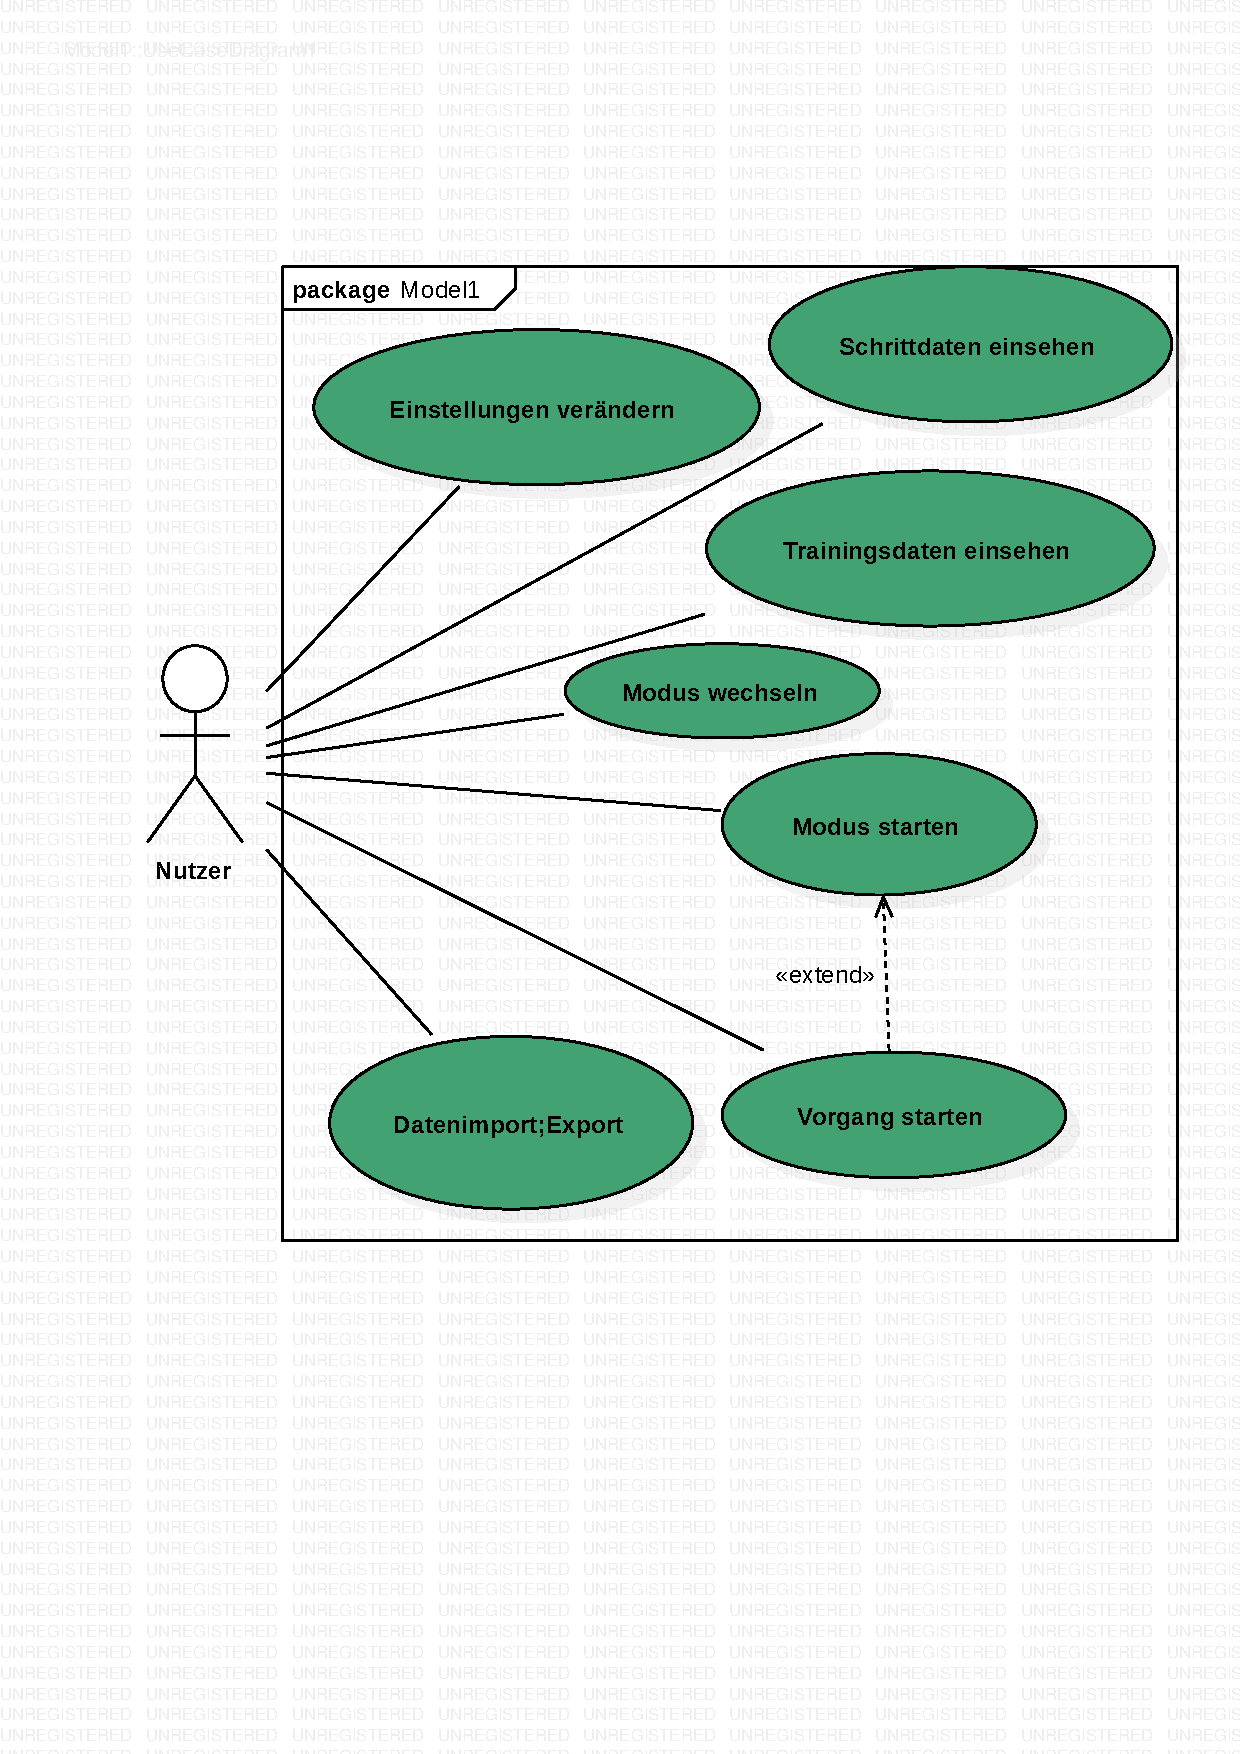
\includegraphics[width=0.8\textwidth]{Vorlaeufiges Use-Case Diagram.pdf}
\end{center}
\section{Benutzeroberfläche}
%%TODO Benni auseinandersetzen
\section{Qualitätszielbestimmungen}
 %%!! Wasn hiermit? Stand noch in der Mail als Unterpunkt. https://www.sosy-lab.org/Teaching/2015-WS-SEP/samples/pflichtenheft.pdf Seite 13 sieht man so eine Tabelle, wie ist das gemeint?
\section{Globale Testfälle und Szenarien}
%%TODO David
  \subsection{Globale Testfälle}
  \subsubsection{Mussanforderungen}
  \paragraph{Schritterkennung beim Gehen}%%bitte Namen der Funktionalen Anf. verwenden!!
  \begin{enumerate}
    \item Das Smartphone wird per Bluetooth mit den Kopfhörern verbunden.
    \item Die App wird gestartet.
    \item Nach dem Startvorgang der App wird in den Modus \glqq Laufmodus\grqq{}(/F100/) gewechselt.
    \item Die Kopfhörer werden korrekt am Ohr des Nutzers angebracht.
    \item Die App zeigt dem Nutzer den Status \glqq stehend\grqq{} an.
    \item Sobald der Nutzer anfängt zu gehen zeigt die App \glqq gehend\grqq{} an.
    \item Sobald der Nutzer wieder still steht ändert sich der Zustand wieder zurück zu \glqq stehend\grqq. 
  \end{enumerate}

  \paragraph{Start/Stop Musikmodus}
  \begin{enumerate}
    \item Das Smartphone wird per Bluetooth mit den Kopfhörern verbunden.
    \item Der Nutzer spielt Musik mit der vorinstallierten Musik-App ab.
    \item Die App wird gestartet.
    \item Nach dem Startvorgang der App wird in den Modus \glqq Start/Stop Musikmodus\grqq{} (/F210/) gewechselt.
    \item Die Kopfhörer werden korrekt am Ohr des Nutzers angebracht.
    \item Der Nutzer beginnt zu gehen.
    \item Der Nutzer startet den gewählten Modus.
    \item Der Nutzer hört auf zu gehen.
    \item Die Musik wird pausiert.
    \item Der Nutzer geht weiter.
    \item Die Musik startet automatisch wieder.
  \end{enumerate}

  \subsubsection{Schritterkennung beim Gehen}
  %%vielleicht ohne absätze als Fließtext? -valle
    \begin{itemize}
    \item[]Das Smartphone wird per Bluetooth mit den Kopfhörern verbunden.
    \item[]Die App wird gestartet.
    \item[]Nach starten der App wird in den Modus \glqq Datenanzeige gehen/stehen\grqq{} gewechselt.
    \item[]Die Kopfhörer werden korrekt am Ohr des Nutzers angebracht.
    \item[]Die App zeigt dem Nutzer den Status \glqq stehend\grqq{} an.
    \item[]Sobald der Nutzer anfängt zu gehen zeigt die App \glqq gehend\grqq{} an.
    \item[]Sobald der Nutzer wieder still steht ändert sich der Zustand wieder zurück zu \glqq stehend\grqq. 
  \end{itemize}
  \subsubsection{Schritte zählen}
  \begin{itemize}
    \item[]
    \item[] 
  \end{itemize}
  \subsection{Szenarien}
    \subsubsection{Bibliotheksnutzung}


\section{Entwicklungsumgebung}
TODO valle

Wir arbeiten an dem Projekt mit Visual Studio 2019, sodass alle eine einheitliche Entwicklungsumgebung verwenden.
%%TODO vllt noch mal diskutieren:
Dabei kommt der .NET Standard 2.0 zum Einsatz, der C\# 7.2 verwendet. Wir arbeiten außerdem mit Xamarin Forms.

Zur Versionskontrolle und zur Projektübersicht wird Git verwendet, das Repository liegt öffentlich auf Github\footnote{\url{https://github.com/vlle1/earablesKIT}}.
\clearpage
\printglossaries
\stepcounter{section}
\end{document}
